% Copyright (c) 2008-2009 solvethis
% Copyright (c) 2010-2016,2018-2019,2021 Casper Ti. Vector
% Copyright (c) 2021 Kurapica
% Copyright (c) 2021 iofu728
% Overleaf version.

%*********************************************************************
% iofu728-pkuthss: 北京大学研究生学位论文模板
% 2021/06/09 v1.0.0
%
% 重要提示:
%   1. 当前overleaf版符合2021研究生学位论文要求,可通过图书馆审核
%   2. 当前版本基于pkuthss v1.9.0
%   3. 请使用UTF-8编码,XeLaTeX方式编译
%   4. 请仔细阅读用户文档
%   5. 修改、使用、发布本文档类请务必遵循LaTeX Project Public License和知识共享4.0
%   6. 如有疑问github/iofu728/pkuthss上提问或联系作者@iofu728
%*********************************************************************

\documentclass[fontset=fandol,ugly]{pkuthss}
  % 学位论文模式  ugly    (默认打开,请保留)
  % 盲审模式      blind   (默认关闭)
  % 字体库        fontset
  %   auto | windows | windows@overleaf | mac | fandol | ubuntu | none
  % windows*, mac为商业字体,如需使用请遵循相应版权协议(默认下overleaf中不可用)
  % fandol与windows效果相近,但字符库偏少,推荐使用(默认);
  % ubuntu字体效果偏差较大; 设为none时需自行配置字体集;

\usepackage[backend=biber,style=gb7714-2015]{biblatex}
  % 参考文献遵循GB/T 7714-2015标准,使用biblatex-gb7714-2015 宏包。
  % 此处使用顺序编码制,如使用著者-出版年制则更改为b7714-2015ay。

% 示例文档用包和设定,该段均可移除.
\usepackage{enumitem,fancyvrb}
\usepackage{booktabs,multirow,longtable,makecell} % 表格相关
\RecustomVerbatimEnvironment{Verbatim}{Verbatim}{frame = single, tabsize = 4, fontsize=\footnotesize}
\renewcommand{\v}[1]{\boldsymbol{#1}}
\newcommand\pkg[1]{\textsf{#1}}

% 参考文献边距字体
\setlength{\bibitemsep}{3bp}
\renewcommand*{\bibfont}{\zihao{5}\linespread{1.27}\selectfont}

\pkuthssinfo{
	cthesisname = {密码编码学与网络信息安全期末作业},
 	thesiscover = {密码编码学与网络信息安全期末作业},
	ethesisname = {Homework},
	ctitle = {密码编码学与网络信息安全报告},
	etitle = {Homework},
	%cauthor = {干皓丞}, 
	eauthor = {Kan, Hao-Cheng},
	%studentid = {2101212850},
	teamname = {郑翰浓、干皓丞},
	% 具体时间以教务为准,初稿3月,送审4月,答辩5月,最终6月。
	%date = {\zhdigits{2021}\ \ 年\ \ \zhnumber{6}\ \ 月},
	date = {\zhdigits{2022}\ \ 年\ \ \zhnumber{6}\ \ 月},
	school = {信息工程学院},
	cmajor = {计算机应用技术}, emajor = {通信及信息安全技术},
	direction = {通信及信息安全技术},
	%mentorlines = {2}, % 导师个数
	mentorlines = {1}, % 导师个数
	% 副教授 A.P. 讲师 Lec.
	cmentor = {朱跃生\ \ 教授}, ementor = {Prof.\ XXX },
	%cmentor = {XXX\ \ 教授\\YYY\ \ 教授}, ementor = {Prof.\ XXX and Prof.\ YYY},
	ckeywords = {信息安全},
	ekeywords = {A,B,C,D},
	% 盲审模式参数, 需在documentclass增加blind
	blindid = {XXXXXXXXX}, discipline = {XXXX}
}
\addbibresource{ref.bib}

\begin{document}
	\frontmatter
	\pagestyle{empty}
	\maketitle
	\cleardoublepage
	% 需替换门户版权声明pdf
	%% Copyright (c) 2008-2009 solvethis
% Copyright (c) 2010-2017,2021 Casper Ti. Vector
% Copyright (c) 2021 iofu728
% All rights reserved.
%
% Redistribution and use in source and binary forms, with or without
% modification, are permitted provided that the following conditions are
% met:
%
% * Redistributions of source code must retain the above copyright notice,
%   this list of conditions and the following disclaimer.
% * Redistributions in binary form must reproduce the above copyright
%   notice, this list of conditions and the following disclaimer in the
%   documentation and/or other materials provided with the distribution.
% * Neither the name of Peking University nor the names of its contributors
%   may be used to endorse or promote products derived from this software
%   without specific prior written permission.
%
% THIS SOFTWARE IS PROVIDED BY THE COPYRIGHT HOLDERS AND CONTRIBUTORS "AS
% IS" AND ANY EXPRESS OR IMPLIED WARRANTIES, INCLUDING, BUT NOT LIMITED TO,
% THE IMPLIED WARRANTIES OF MERCHANTABILITY AND FITNESS FOR A PARTICULAR
% PURPOSE ARE DISCLAIMED. IN NO EVENT SHALL THE COPYRIGHT HOLDER OR
% CONTRIBUTORS BE LIABLE FOR ANY DIRECT, INDIRECT, INCIDENTAL, SPECIAL,
% EXEMPLARY, OR CONSEQUENTIAL DAMAGES (INCLUDING, BUT NOT LIMITED TO,
% PROCUREMENT OF SUBSTITUTE GOODS OR SERVICES; LOSS OF USE, DATA, OR
% PROFITS; OR BUSINESS INTERRUPTION) HOWEVER CAUSED AND ON ANY THEORY OF
% LIABILITY, WHETHER IN CONTRACT, STRICT LIABILITY, OR TORT (INCLUDING
% NEGLIGENCE OR OTHERWISE) ARISING IN ANY WAY OUT OF THE USE OF THIS
% SOFTWARE, EVEN IF ADVISED OF THE POSSIBILITY OF SUCH DAMAGE.

% 此处不用 \specialchap,因为学校要求目录不包括其自己及其之前的内容。
\chapter*{版权声明}
% 综合学校的书面要求及 Word 模版来看,版权声明页不用加页眉、页脚。
\thispagestyle{empty}

任何收存和保管本论文各种版本的单位和个人,
未经本论文作者同意,不得将本论文转借他人,
亦不得随意复制、抄录、拍照或以任何方式传播。
否则一旦引起有碍作者著作权之问题,将可能承担法律责任。

% 替换门户下载pdf
\begin{textblock}{1}(-0.8,-0.08)
    \colorbox{white}{
        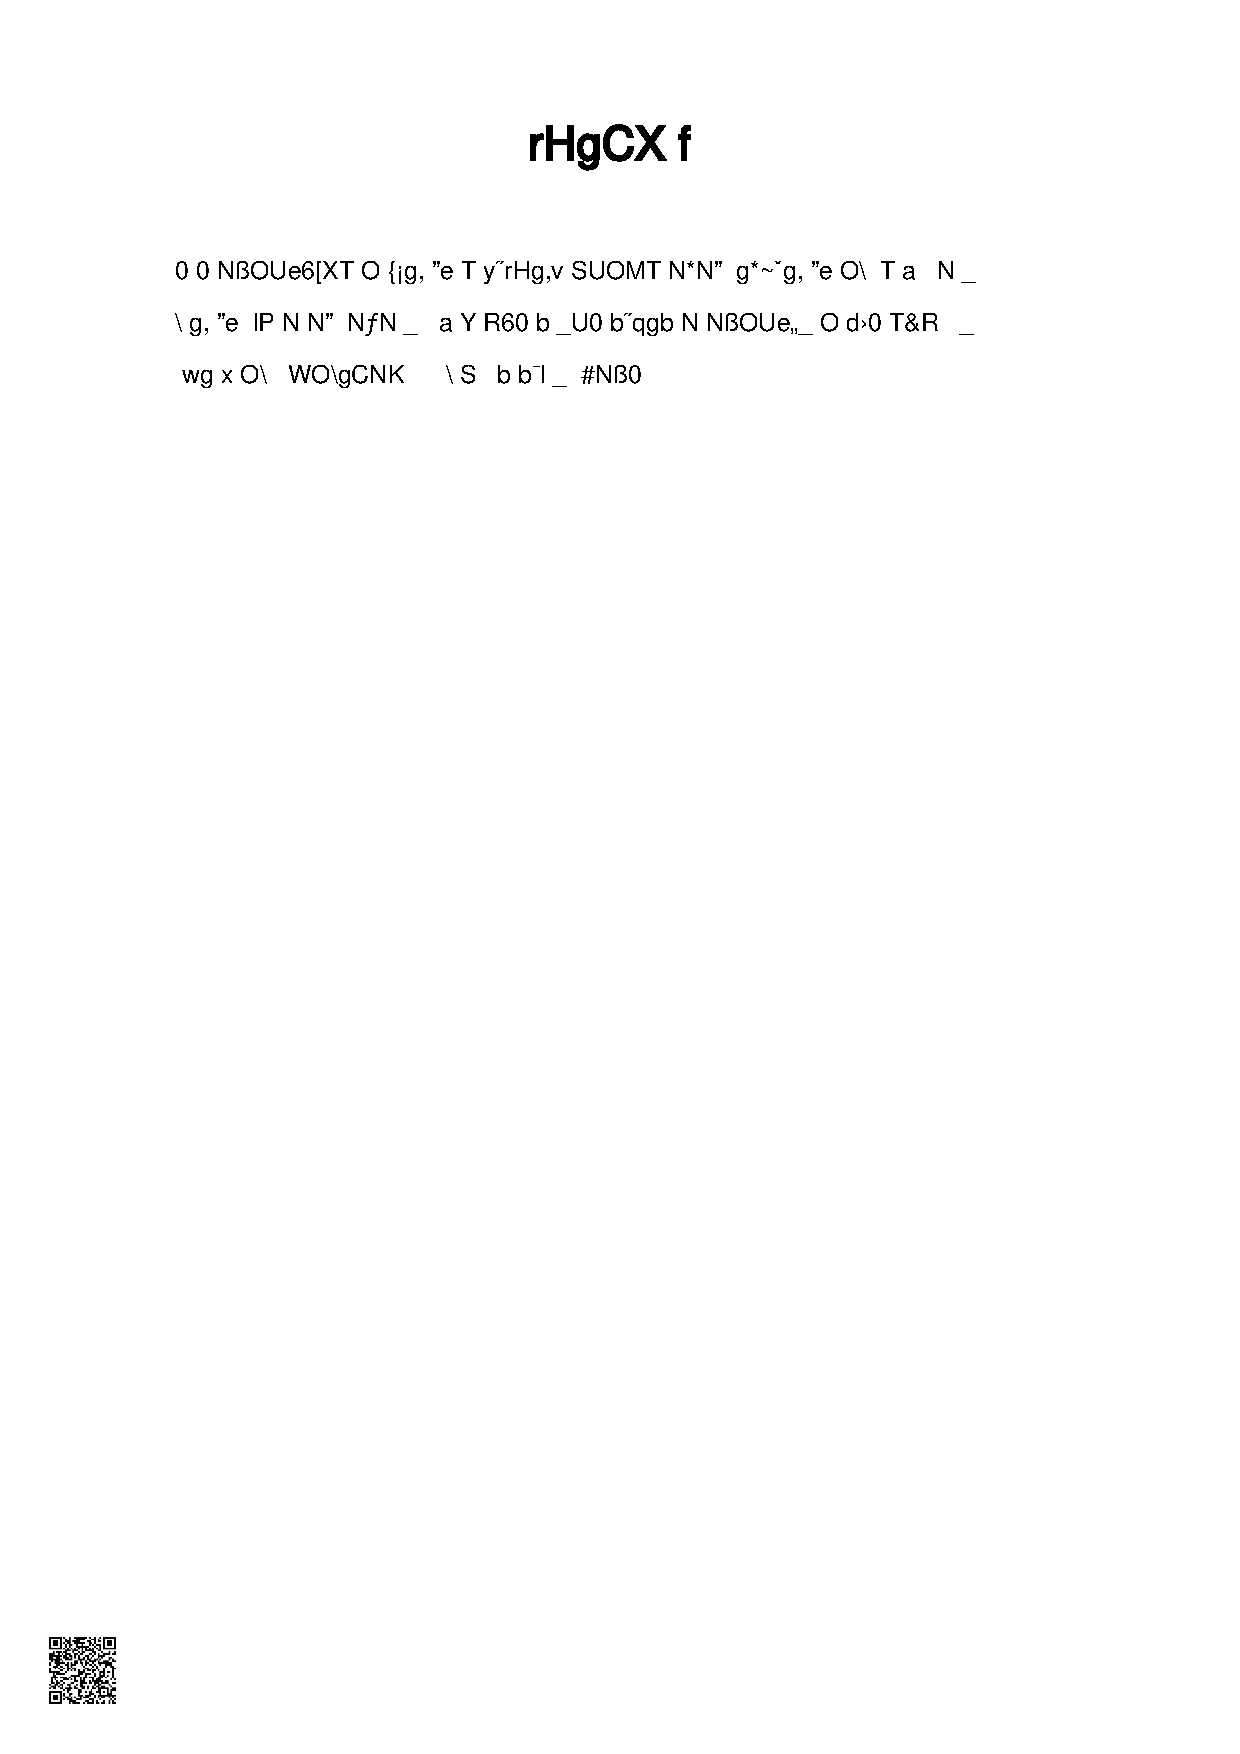
\includegraphics[height = 1.2448\textheight]{img/bqsm_180xxxxxxx.pdf}
    }
\end{textblock}

% vim:ts=4:sw=4

	\cleardoublepage
	\pagestyle{plain}
	\setcounter{page}{0}
	\pagenumbering{Roman}
	\begin{cabstract}

XXXXX


\end{cabstract}

%\begin{eabstract}
%    英文摘要部分...
%\end{eabstract}

% vim:ts=4:sw=4

	\tableofcontents
	% 如有需要使用主要符号对照表
	\begin{denotation}

\item[$x,y,m,n,t$] 标量,通常为变量
\item[$K,L,D,M,N,T$] 标量,通常为超参数
\item[$x\in \mathbb{R}^{D}$] D维列向量
\item[$(x_1,\cdots,x_D)$] D维行向量
\item[$(x_1,\cdots,x_D)^T$ or $(x_1;\cdots;x_D)^T$]  D维行向量
\item[$x\in \mathbb{R}^{KD}$]  ($KD$)维的向量
\item[$\mathbb{M}_i$ or $\mathbb{M}_i(\v x)$]  第$i$列为$\v 1$(或者$\v x$),其余为$\v 0$的矩阵
\item[$diag(\v x)$]  对角矩阵,其对角元素为$\v x$
\item[$\v I_N$ or $I$]  ($N\times N$)的单位阵
\item[$\v A \in \mathbb{R}^{D_1\times D_2\times \cdots \times D_K}$]  大小为$D_1\times D_2\times \cdots \times D_K$的张量
\item[$\{x^{(n)}\}^{N}_{n=1}$]  集合
\item[$\{(x^{(n)},y^{(n)})\}^{N}_{n=1}$]  数据集
\item[$\mathcal{N}(\v x;\mu,\sum)$]  变量$x$服从均值为$\mu$,方差为$\sum$的高斯分布

\end{denotation}

\footnotetext[1]{本符号对照表内容选自\citeauthor{qiu2020nndl}老师的《神经网络与深度学习》\cite{qiu2020nndl}一书。}


	\mainmatter
	\chapter{深度伪造在生成与检测跟对抗性}
\label{chap:1}

本作业因个人信息隐私保护的原因,对其深度伪造与检测跟对抗性等工作做出简化的工作梳理,其包含了多模态多尺度(Multi-modal Multi-scale) 和增量学习 (Incremental Learning) 的近期深度伪造在检测的工作,其二则是包含了语音检测对抗性跟应对语音攻击的深度伪造在语音检测与对抗性部分,其三则是深度伪造在生成与检测的对抗性,此又分为生成的对抗性与检测的对抗性,最后则是区块链进行视频追踪的手段,作为在深度伪造与检测跟对抗性领域的安全措施。

\section{近期深度伪造在检测的工作}

近来两篇重要的研究一个是 Wang, J 等人 \cite{wang2021m2tr} 在其发表的 M2TR: Multi-modal Multi-scale Transformers for Deepfake Detection 所提出多模态多尺度。跟 Khan, S. A 等人 \cite{khan2021video} 提出了一种增量学习策略,可以在更少量的资料上微调所提出的模型,并实现更好的深度伪造检测性能。对各种公共 Deepfake 数据集的综合实验表明,所提出的具有增量学习的视频转换器模型通过对序列数据的增强特征学习,在 Deepfake 视频检测任务中实现了最先进的性能。

\subsection{多模态多尺度的 M2TR}

Wang, J 等人 \cite{wang2021m2tr} 在其发表的 M2TR: Multi-modal Multi-scale Transformers for Deepfake Detection 中说明,Deepfake 技术所产生的伪造图像广泛传播对数位资讯的可信度构成了严重威胁,这需要有效的方法来检测由先进技术所生成具有感知力的 Deepfake 成果。大多数现有方法通过将输入图像对应到二进制预测而不捕获不同像素之间的一致性来使用深度神经网络来对抗 Deepfakes 技术。在该研究中,研究者旨在为 Deepfake 检测捕获不同尺度的细微操作伪影,并通过转换器模型实现了这一点,该模型最近在为计算机视觉中的各种识别任务建模像素之间的依赖关系方面表现出卓越的性能。同时研究者介绍了一种多模态多尺度变换器(M2TR),它使用多尺度变换器对不同大小的补丁进行操作,以检测不同空间级别的局部不一致性,为了改善检测结果并增强我们方法对图像压缩的鲁棒性,M2TR 还获取频率信息,并使用交叉模态融合模块将其与 RGB 特征进一步结合。开发和评估 Deepfake 检测方法需要大规模的数据集。此研究观察到现有基准中的样本包含严重的伪影并且缺乏多样性,这促使此研究引入了一个高品质的 Deepfake 资料集 SR-DF,它由 4,000 个由最先进的面部交换和面部重演方法去生成的 DeepFake 组成影像,最后在三个 Deepfake 资料集上,研究者进行了广泛的实验来验证所提出方法的有效性,该方法优于最先进的 Deepfake 检测方法。

另外从研究中的说明可以看到其研究展示,现有数据集中伪造图像的视觉伪影,包括颜色不匹配 (row 1 col 1, row 2 col 3,
row 3 col 1, row 3 col 2, row 3 col 3) 、形状失真 (row 1 col 3, row 2 col 1)、可见边界 (row 2 col 2) 和脸部模糊 (row 1 col 2, row 4 col 1, row 4 col 2, row 4 col3)。

\begin{figure}[htb]
\centering 
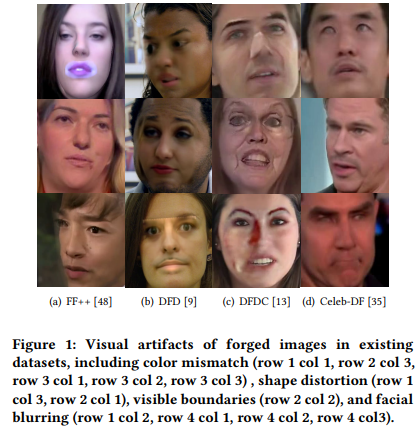
\includegraphics[width=0.50\textwidth]{img/p1m1.png} 
\caption{数据集中伪造图像的视觉伪影}
\label{Test}
\end{figure}

此外该研究提出了一种名为 M2TR 的多模态多尺度变压器 ,首先运用 CNN 模型提取特征,然后生成作为 Transformer 模型的输入,用于捕捉不同区域在多尺度上的不一致性,并在此基础上增加了频域信息,融合后输出结果。

\begin{figure}[htb]
\centering 
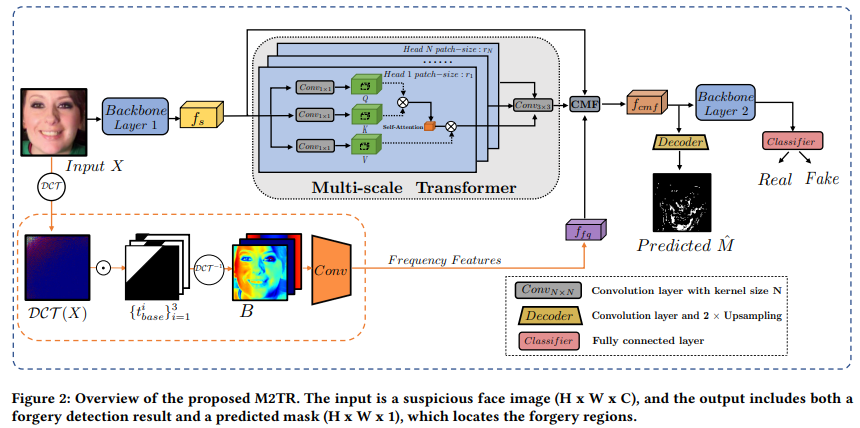
\includegraphics[width=0.90\textwidth]{img/p1m2.png} 
\caption{Multi-scale Transformer 架构}
\label{Test}
\end{figure}

\subsubsection{离散余弦变换(DCT)}

DCT 也就是离散余弦变换的缩写,将图像从空域转化到频域,其研究者认为,图像的低频信息集中在 0-1/16 部分,中频信息集中在 1/16-1/8,剩下的部分是图像的高频信息,通过构造三个滤波器来完成提取低中高频信息。通过经过 DCT 变换后的图像中黑色的部分而舍弃白色的部分,从而得到提取低频,中频,高频信息。并用将得到的信息进行逆变换,将低中高频信息组合在一起,作为频域信息的输入,送入卷积网络中,将其输出作为提取到的频域特征。

\subsubsection{Multi-scale Transformer}

希望定位篡改伪影与其他区域不一致,因此需要建模长期关系,计算相似度,引入多尺度的 Transformer,来覆盖不同大小的区域。输入图片再 backbone 提取 shallow feature,然后分成不同的大小去计算 patch-wise 的 self attention,也就是每个 Patch(rh*rh*c)展开成一维向量,使用 FC 层 embed 到 Query Embeddings,同样得到 k 和 v,最后通过矩阵相乘得到相速度最后通过 Softmax 输出。

$$
\alpha_{i, j}^{h}=\operatorname{softmax}\left(\frac{\boldsymbol{q}_{i}^{h} \cdot\left(\boldsymbol{k}_{j}^{h}\right)^{T}}{\sqrt{r_{h} \times r_{h} \times C}}\right), 1 \leq i, j \leq N
$$

最后相乘相加得到查询 Patch 的输出:

$$
\boldsymbol{o}_{i}^{h}=\sum_{j=1}^{N} \alpha_{i, j}^{h} v_{j}^{h}
$$

接收所有输出 Sitch and Reshape 原本的 Resolution,不同的头拼接通过 Residual Block 得到输出结果。

$$
f_{m t} \in \mathbb{R}(H / 4) \times(W / 4) \times C
$$

这一部分与视觉注意力机制类似,唯一的区别是,这一部分使用多种不同尺度的 Patch 对图像进行采样。举个例子,假设使用的是分辨率为 56 * 56 的图像,一般的视觉注意力机制会使用 14 * 14 的 Patch 对图像进行采样,采样后将图片分为 4 * 4 也就是 16 个块,随后再对这16个块进行编码,得到 16 个 token,最后使用自注意力机制,通过每个串得到 qkv,最后得到输出结果。

而所谓的多尺度是将这一过程重复数次,每次使用的 Patch 大小不同,第一次我们使用与图像相同大小的 Patch,采用后得到 1 个块。第二次使用 28 * 28 大小的 Patch,得到 2 * 2 也就是 4 个块。第三次使用 14 * 14 大小的 Patch,得到 4 * 4 = 16 个块,最后使用 7 * 7 大小的 Patch,得到 8 * 8 = 64 个块。每一个尺度都会再各自尺度分别利用自注意力机制进行计算,得到各自尺度的输出结果,最后将各个输出结合再一起,送入卷积中,得到 Transformer 部分的特征提取。


\subsubsection{多头自注意力 (Mutil-head Self Attention, MSA)}

另外再详细说明单个多头自注意力 (Mutil-head Self Attention, MSA) 的操作过程。在 VIT 中,首先将图片按照一定的尺寸进行分割,变成一个个 Token,举例来说,当输入图片是 224 * 224, 而 Patch 大小为 16 * 16,就会得到 14 * 14 也就是 196 个块。随后将每个块放入 embed 模块,映射成 196 个 Token,每个 Token 的长度被规定为 768(14 * 14 * 3)。这时图片从 [b, 3, 224, 224] 变成了 [b, 196, 768]。然后此时需要增加一个 cls 和一个位置信息 pos,所谓的 cls 是一个特殊字符,它的具体作用是用于分类,在 nlp 中 cls 通常位于第一位,位置信息表示每一个 Token 的位置,由于改变 Token 的位置会将整张图片的语义信息改变,所以添加位置信息是必要的。 cls 的大小是 [b, 1, 768], 位置信息的大小是 [ b, 197, 768],至于是用 197 的原因呢,是因为在原始 Token 的基础上会将 cls 与 Token 进行 concatenate,从而使 Token 的大小变成了 [b, 196+1, 768],然后将 Token 与位置信息相加,而不是 concatenate,这样就完成了 embed 操作。 Embed 完成后,我们将 Token 送入到 ATTENTION 中,同时为了并行计算,此工作会直接使用 nn.Linear, 将输出从 [b, 197, 768] 变成 [b, 197, 3*768],然后 reshape 成 [3,b, 197, 768],依次得到 qkv,然后按照 VIT 论文中的计算公式,得到输出结果。此时要注意的地方在于,如果是有多个头部,那么得到的 qkv 应该是 [3,b, head\_num, 197, 768/head\_num],所有的操作分成多个头部进行,得到的输出再拼接在一起,但由于此工作是并行计算,所以最后得到的输出应该是 [b, head\_num, 197, 768/head\_num],然后直接 reshape 变成 [b, 197, 768]就完成了全部操作。在该问题中,由于是使用 Transformer 来提取特征图,而非直接分类,所以并不需要使用 cls token,并且这样也方便后续处理工作。

\begin{figure}[htb]
\centering 
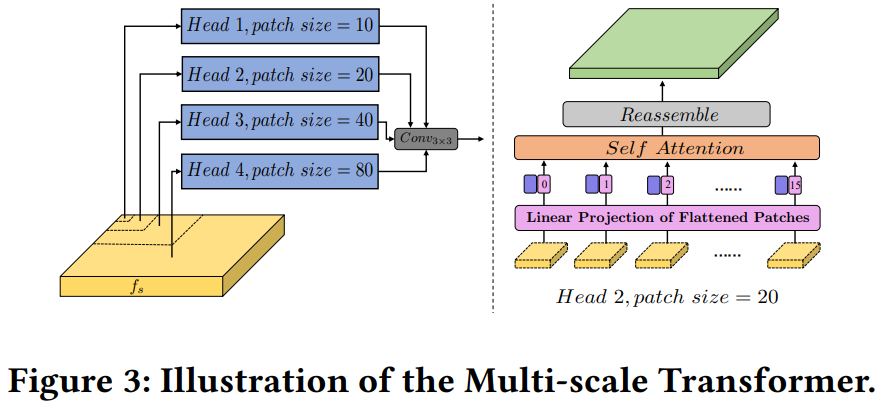
\includegraphics[width=0.90\textwidth]{img/p1m3.png} 
\caption{Multi-scale Transformer 说明}
\label{Test}
\end{figure}

\subsubsection{Cross Modality Fusion}

CMF 模块是一个特征融合模块,将上述三个模块的输出融合再一起。具体的操作与一个多头自注意力机制类似,而与 MSA 相似地方在于,CMF 模块中也存在 qkv ,其 q 是通过空域特征图卷积得到,k 和 v 是通过频域特征图卷积得到。首先按照 MSA 算法将空域特征图和频域特征图融合,具体的计算公式如下所示。

$$
\begin{aligned}
&Q=\operatorname{Conv}_{q}\left(f_{s}\right), K=\operatorname{Conv}_{k}\left(f_{f q}\right), V=\operatorname{Conv}_{v}\left(f_{f q}\right) \\
&f_{\text {fuse }}=\operatorname{softmax}\left(\frac{Q K^{T}}{\sqrt{H / 4 \times W / 4 \times C}}\right) V
\end{aligned}
$$

得到的融合特征 $f_{fuse}$ 在和空域特征和 Transformer 输出的特征图相加,作为特征图送入卷积网络中进一步提取特征。其具体的计算公式如下。

$$
f_{c m f}=C o n v_{3 \times 3}\left(f_{s}+f_{m t}+f_{f u s e}\right)
$$


\subsection{增量学习}

Khan, S. A 等人 \cite{khan2021video} 在其发表的 Video Transformer for Deepfake Detection with Incremental Learning 工作中说明了,Deepfake 的面部伪造在互联网上广泛传播,这引起了严重的社会担忧,在该研究中,研究者提出了一种具有增量学习功能的新型影像转换器,用于检测深度伪造影像,而为了更好地对齐输入人脸图像,我们使用 3D 人脸重建方法从单个输入人脸图像生成 UV 纹理。其对齐的人脸图像还可以提供在 UV 纹理图像中无法感知的姿势、眨眼和嘴巴运动资讯,因此研究者使用人脸图像及其 UV 纹理图来提取图像特征。最后研究者提出了一种增量学习策略,可以在更少量的资料上微调所提出的模型,并实现更好的深度伪造检测性能。对各种公共 deepfake 数据集的综合实验表明,所提出的具有增量学习的视频转换器模型通过对序列数据的增强特征学习,在 deepfake 视频检测任务中实现了最先进的性能。

深度学习的最新发展和大规模数据集的可用性导致强大的深度生成模型可以生成高度逼真的合成视频,同時最先进的生成模型具有大量有利的应用,但生成模型也被用于恶意目的。生成模型的此类应用之一則是深度伪造视频生成,其模型已经发展到难以区分真假视频的程度。此外 Deepfake 可用于不道德和恶意目的,例如传播虚假宣传、冒充政治领导人说或做不道德的事情,以及诽谤无辜的个人。該領域可以分为四类:人脸替换、人脸再现、人脸编辑和完整的人脸合成。另外要注意的地方在於 Deepfake 生成技术呈指数级增长,并且变得越来越难以检测,当前的检测系统不能有效地检测被操纵的介质。而在 Deepfake 检测挑战赛 (DFDC) 中,模型在未见过的数据上进行测试时的性能比在 DFDC 测试集上的性能差得多。

重要的地方在於泛化能力是现有深度伪造检测系统的主要关注点之一,各种各样的检测系统使用 CNN 和循环网络来检测被操纵的媒体。Li et al. 使用 CNN 来检测来自 Deepfake 数据集的图像中的面部扭曲伪影,其所提出的方法在存在可见的面部扭曲伪影的情况下效果很好。另外大多数 Deepfake 生成技术采用后处理程序来去除翘曲伪影,这使得检测 Deepfake 视频变得更加困难。现有方法的另一个限制是,大多数提出的系统对视频中的帧进行预测并对预测进行平均以获得整个视频的最终预测分数。所以它没有考虑框架之间的关系。而为了克服这个问题,該研究者提出了一种新颖的视频转换器来提取具有时间信息的空间特征。

Vaswani et al. 在  Attention is All you Need. 中首次提出了 Transformer 用于自然语言处理任务。自那时起,Transformer 在自然语言处理任务中表现出强大的性能,例如机器翻译、文本分类、问答和自然语言理解,而广泛使用的变压器架构包括来自变压器的双向编码器表示 (BERT)、鲁棒优化的 BERT 预训练 (RoBERTa)、生成式预训练变压器 (GPT) v1-v3。Transformer 模型可以自然地容纳用于特征学习的视频序列,为了提取更多信息特征,研究者在对齐的面部图像及其相应的 UV 纹理图上训练我们的模型。

现有方法使用对齐的 2D 人脸图像,这样的对齐方式只是将人脸居中,而不考虑人脸是否正面。当人脸未正面化时,相机未捕捉到的面部部分会导致面部信息丢失,并与正面化的人脸图像错位。同時使用 UV 纹理,所有面部图像都对齐到从生成的 3D 面部创建的 UV 贴图中。同時由于生成的 3D 人脸覆盖了所有的人脸部位,因此没有信息丢失,在 UV 贴图中,所有面部的面部部分可以位于相同的空间空间中。比如所有的鼻子部分都位于 UV 贴图上的同一区域,所以 UV 贴图中的面可以更好地对齐,另外为了处理人脸图像和 UV 纹理图的输入组合,我们在输入数据结构中使用可学习的片段嵌入。而段嵌入有助于模型区分同一数据结构中不同类型的输入。此外,該研究的研究者使用增量学习策略在不同数据集上逐步调整此研究的模型,以在新数据集上实现最先进的性能,同时保持先前数据集上的性能。

其贡献可以概括为三方面:其一,提出了一种带有人脸 UV 纹理图的视频转换器,用于深度伪造检测。在 ve 不同的公共数据集上的实验结果表明,此方法比最先进的方法实现了更好的性能。其二,所提出的段嵌入使网络能够提取更多信息特征,从而提高检测精度。其三,所提出的增量学习策略提高了所提出模型的泛化能力。在综合实验表明,此研究的模型可以在新数据集上取得良好的性能,同时保持其在以前数据集上的性能。

\begin{figure}[htb]
\centering 
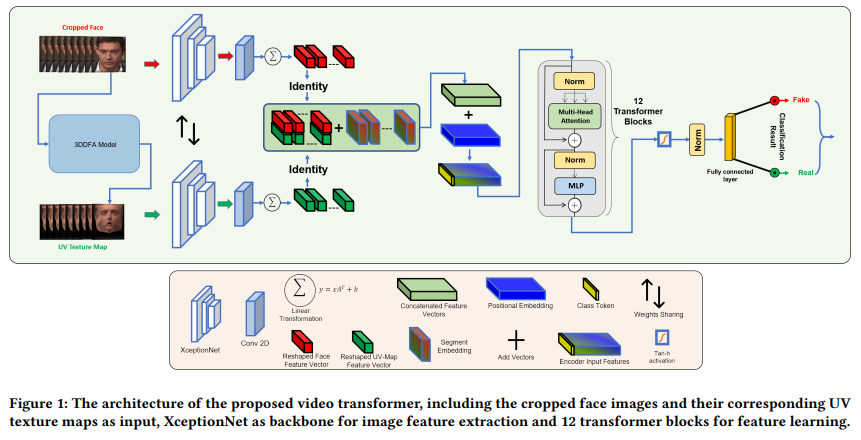
\includegraphics[width=0.90\textwidth]{img/p3m1.png} 
\caption{视频转换器的架构}
\label{Test}
\end{figure}

要注意的地方在于,研究中所提出的视频转换器的架构,包括作为输入的裁剪后的人脸图像及其对应的 UV 纹理图,作为图像特征提取骨干的 XceptionNet 和用于特征学习的 12 个转换器块。該研究所建议的增量学习策略的说明,當中的 D1 代表用于训练模型的真实数据,而 D2 由 FaceSwap 和 Deepfakes 数据集组成,此外 D3 代表 Face2Face 数据集,D4 代表神经纹理数据集。而 D5 和 D6 代表 DFDC 数据集,最後 D7 代表 DeepFake Detection (DFD) 数据集。

\begin{figure}[htb]
\centering 
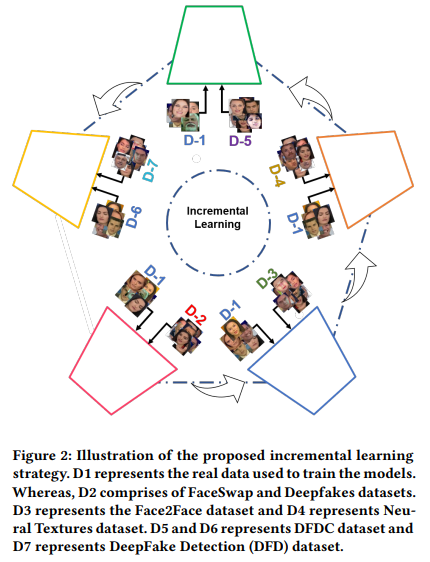
\includegraphics[width=0.50\textwidth]{img/p3m2.png} 
\caption{增量学习策略的说明}
\label{Test}
\end{figure}

\section{深度伪造在语音检测与对抗性}

\subsection{语音检测对抗性}

Huang, C. Y 等人 \cite{9383529},在其 Defending Your Voice: Adversarial Attack on Voice Conversion 中说明了,近年来在语音转换方面取得了实质性的改进,将一个话语的说话者特征转换为另一个说话者的特征,而不改变话语的语言内容。尽管如此,改进的转换技术也导致了对隐私和身份验证的担忧。因此,非常希望能够通过这种语音转换技术来防止一个人的语音被不当使用。这就是为什么该研究报告了对语音转换执行对抗性攻击的第一次已知尝试,研究者将人类难以察觉的噪音引入说话人的话语中,而说话人的声音要受到保护。鉴于这些对抗性示例,语音转换模型无法将其他话语转换为听起来像是被防御者发出的声音。在两个当前最先进的零样本语音转换模型上进行了初步实验。报告了白盒和黑盒场景中的客观和主观评估结果。结果表明,转换后的话语的说话人特征与被辩护人的说话人特征明显不同,而被辩护人的对抗样本与真实话语没有区别。

语音转换旨在改变话语的某些特定声学特征,例如说话者身份,同时保留语言内容。这类技术通过深度学习变得更加强大,但改进的技术也导致了对隐私和身份验证的担忧,而一个人的身份可能会被语音转换伪造并以不正当的方式被利用,这只是当今观察到的由深度学习产生的许多 deepfake 问题之一,例如合成的假照片或假语音。因此,检测任何此类伪影或防御此类活动变得越来越重要,这同样适用于语音转换。
 
另一方面,众所周知地在于神经网络在存在某些特定噪声的情况下是脆弱的,或者如果输入受到人类无法察觉的细微扰动的干扰,则容易产生不同或不正确的结果。其对抗性攻击是产生可以欺骗神经网络的微妙扰动。它在一些判别模型上取得了成功,但在生成模型上的报导较少。该研究建议对语音转换执行对抗性攻击,以防止一个人的说话者特征被不恰当地用于语音转换。人类难以察觉的扰动被添加到要防御的说话者产生的话语中。提出了三种不同的方法,端到端攻击、嵌入攻击和反馈攻击,使得转换后的话语的说话人特征与防御说话人的说话人特征大不相同。

研究者对两个最近最先进的 zeroshot 语音转换模型进行了客观和主观评估,客观说话人验证表明转换后的话语与被辩护说话人产生的话语有显著差异,然后通过主观相似性测试进行验证。通过更接近真实应用场景的代理模型,还验证了所提出方法的有效性,用于黑盒攻击。

\begin{figure}[htb]
\centering 
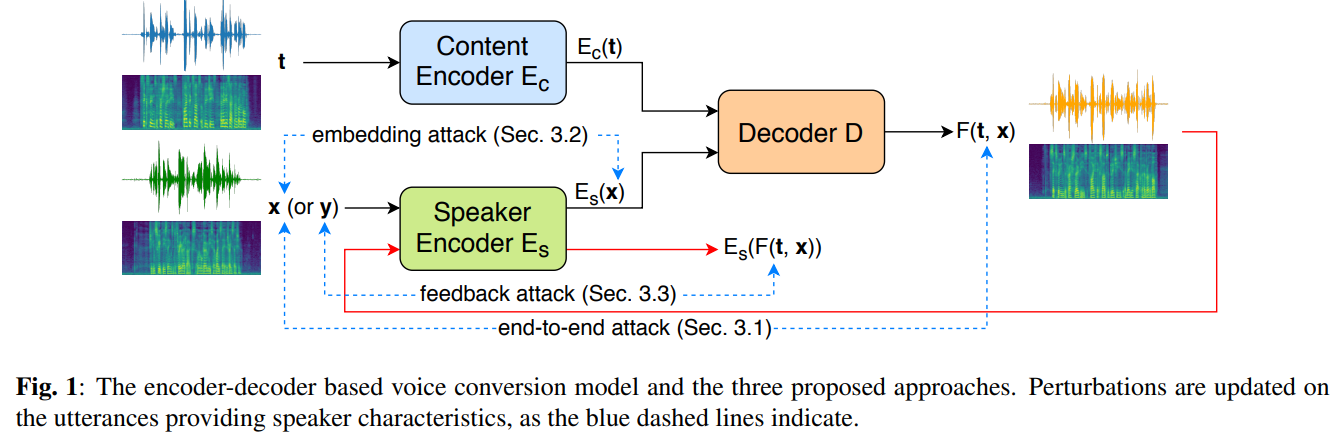
\includegraphics[width=0.90\textwidth]{img/p2m1.png} 
\caption{语音转换模型和三方法}
\label{Test}
\end{figure}

传统上语音转换需要并行数据,或者两个说话者的训练话语必须配对和对齐。为了克服这个问题,Chou et al. 通过对抗训练分别获得语言内容和说话者信息的解耦表示; CycleGAN-VC 使用循环一致性来确保转换后的语音对目标说话者的特征具有语言意义; StarGAN-VC 为多对多语音转换引入了条件输入。零样本方法尝试将话语转换为仅给定一个示例话语而不进行微调的任何说话者,并且目标说话者不一定以前见过。 Chou et al. 为此目的采用了自适应实例规范化; AUTOVC 集成了预训练的 d 向量和编码器瓶颈,实现了最先进的结果。

另外基于编解码器的语音转换模型和提出的三种方法。如蓝色虚线所示,扰动在提供说话者特征的话语上更新。值得注意的地方在于,该研究测试了两个场景。在第一种情况下,攻击者可以完全访问要攻击的模型。有了完整的架构加上模型的所有训练参数可用,我们可以直接应用对抗性攻击。

\begin{figure}[htb]
\centering 
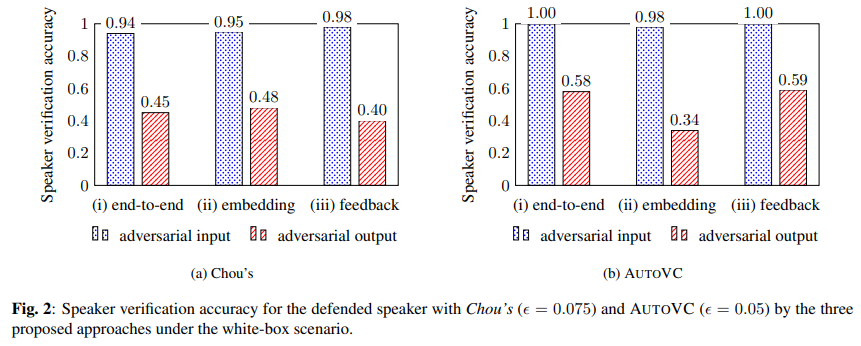
\includegraphics[width=0.90\textwidth]{img/p2m2.png} 
\caption{白盒场景下三种建议方法对 Chou ($\epsilon = 0.075$) 和 AUTOVC ($\epsilon = 0.05$) 的防御说话人的说话人验证准确度}
\label{Test}
\end{figure}

这种场景被称为白盒场景,其中所有实验都是在 Chou 的模型和 AUTOVC 上进行的,并使用它们公开可用的网络参数,并在完全相同的模型上进行评估。第二种被称为黑盒场景,攻击者无法直接访问被攻击模型的参数,甚至可能架构未知。为了攻击 Chou 的模型,我们训练了一个具有相同架构但初始化不同的新模型,而对于 AUTOVC,我们训练了一个新的扬声器编码器,其架构类似于原始 AUTOVC 中的架构。然后将这些新训练的模型用作代理模型,以生成对抗性示例,以与白盒场景相同的方式与公开可用的示例进行评估。图中可以看到白盒场景下三种建议方法对 Chou ($\epsilon = 0.075$) 和 AUTOVC ($\epsilon = 0.05$) 的防御说话人的说话人验证准确度。

\subsection{应对语音攻击}

Zeinali H 等人 \cite{zeinali2019detecting} 所发表的 Detecting spoofing attacks using VGG and SincNet: BUT-Omilia submission to ASVspoof 2019 challenge 的研究成果中,介绍了布尔诺理工大学 (BUT) 和 Omilia 共同努力的系统描述 — ASVSpoof2019 Spoofing and Countermeasures Challenge 的对话智能,其物理访问(PA)的主要提交是两个 VGG 网络的融合,并在单通道和双通道特征上进行了训练。对于逻辑访问 (LA),研究者的主要系统是 VGG 和最近引入的 SincNet 架构的融合,其 PA 上的结果表明,所提出的网络在所有条件下都产生了非常有竞争力的性能,并且与官方基线相比实现了 86\% 的相对改进。另一方面,LA 上的结果表明,尽管所提出的架构和训练策略在某些欺骗攻击上表现得非常好,但它无法推广到在训练期间看不见的某些攻击下。

为了促进更好和更安全的客户支持,例如银行和呼叫中心,对方便和强大的自动身份验证系统的需求不断增长,自动说话人验证 (ASV) 又名语音生物识别技术可以说是此类应用中最自然且侵入性最小的身份验证方法。不幸的是此 ASV 系统容易受到由文本到语音 (TTS) 和语音转换 (VC) 方法创建的合成语音以及重放/演示攻击的攻击。通过这种方法欺骗 ASV 系统的尝试被称为 ASV 欺骗攻击。虽然 ASV 的研究已经进行了几十年,但直到近几年,研究界才开始通过一系列 ASV 欺骗和对策挑战系统地解决欺骗攻击。

针对 ASV 系统的欺骗攻击可分为 4 种类型。第一个是模拟,可以被准确的 ASV 系统拒绝,第二种和第三种类型是 TTS 和 VC,它们在 ASVspoof 2015 挑战中得到解决,并且已经提出了几种检测它们的方法。最后一种攻击是使用预先录制的音频进行重放攻击,它被认为是最难检测的攻击。解决这个问题的可能方法是(a)基于检测录制和重放音频中的典型失真的反欺骗技术,(b) 使用音频指纹检测注册话语的重放,以及 (c)使用活跃度检测和短语验证在依赖于文本的说话者验证中。

作为 2019 年自动说话人验证 (ASV) 反欺骗挑战的一部分,该研究介绍了 BUT 和 Omilia 为最后三种攻击类型引入新对策的合作努力。所有的系统都基于深度神经网络 (DNN) 架构,经过训练可以区分真实语音和合成或重放语音,并用作端到端分类器,即没有任何外部后端。物理访问 (PA) 系统是两个使用不同特征的 VGG 网络的融合,而逻辑访问 (LA) 系统是一个 VGG 网络和两个 SincNet 网络的融合。

\begin{figure}[htb]
\centering 
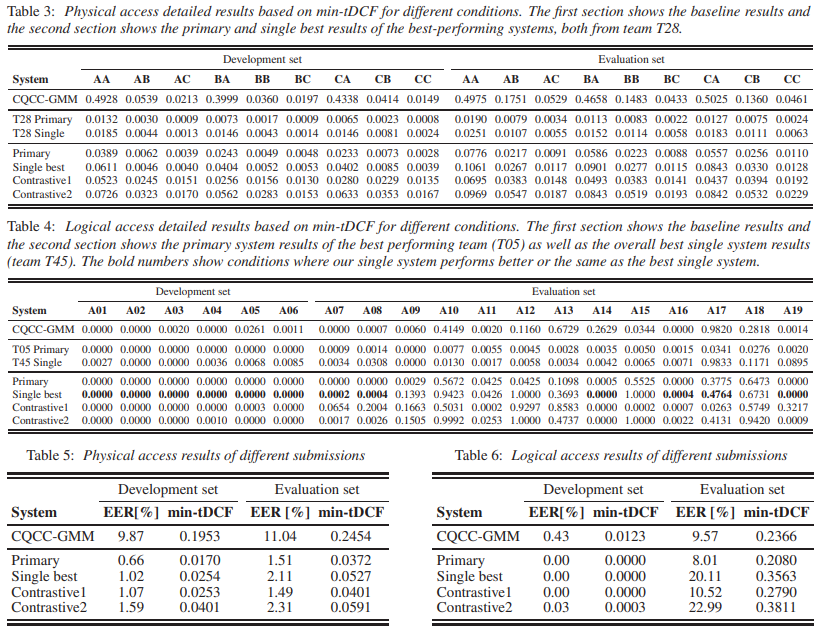
\includegraphics[width=0.90\textwidth]{img/p4m1.png} 
\caption{研究结果}
\label{Test}
\end{figure}

\subsubsection{特征和预处理 (Features and preprocessing)}

对于这个挑战,该研究探索了几个特征,例如梅尔滤波器组(Mel-filter bank)、MFCC、恒定 Q 变换 (constant Q-transform; CQT)、CQCC 和功率谱图(Power Spectrogram),在探索的特征中,功率谱图产生了优越的性能,其次是 CQT 特征。该研究在大多数实验中都使用这两个特征。特别是提交的系统使用功率谱图作为单个输入通道,或者将功率谱图和 CQT 特征作为两个不同的输入通道馈送。作为特征预处理,CQT 和功率谱图都首先被转移到对数域,然后在被馈送到网络之前进行均值和方差归一化(MVN)。

\subsubsection{用于网络训练的示例和小批量生成}

生成训练示例和小批量的过程会极大地影响神经网络在音频处理中的性能。因此该研究为此尝试了几种不同的策略。例如生成研究者首先连接同一类 (相同攻击 id)和说话者的所有特征,然后将连接的特征分成相同大小的小段。最初使用了 4 秒的片段,但在进行了几次实验后,发现在较小片段上训练的网络比在大片段上训练的网络表现更好,主要是因为它们对训练数据的过度拟合较少。用于训练提交系统的示例大小为一秒(即 100 帧)。对于小批量生成,研究者尝试了将示例分配到小批量的不同策略。发现最好的策略是在每个 minibatch 中只使用来自单个说话者的示例 (一些 minibatch 可能包含来自更多说话者的示例,以便使用所有训练数据)。每个 minibatch 有 128 个样本。在每个 epoch 之后,将示例随机化并再次生成 minibatch 以进行更好的泛化。

\subsubsection{Training and development data}

为了训练网络使用了挑战的官方训练集,该集合包含来自 20 个扬声器的音频样本。其中一位发言者被随机选择用于网络训练验证集,该验证集大约是训练数据的 5\%,其开发集也是官方挑战的开发集,这组包含 20 个扬声器,仅用于评估网络和比较不同的方法和训练策略。

\subsubsection{Networks and training strategies}

对于这一挑战,物理访问使用了两种不同的拓扑。第一个是 VGG 网络的修改版本,它在音频标记和音频场景分类方面表现出良好的性能,第二个网络是 Light CNN (LCCN) 的修改版本,在 ASVSpoof2017 挑战赛中表现最佳。该研究在 2019 年声学场景分类挑战赛中使用了这两个网络的修改版本。

1. 类 VGG 网络 (VGG-like network)

VGG 网络包括几个卷积层和池化层,然后是一个统计池和几个执行分类的密集层。研究中提供了对所提议的 VGG 架构的详细描述。模型中有 6 个卷积块,每个包含 2 个卷积层和一个最大池,每个最大池化层将频率轴的大小减小到一半,而其中只有一个会降低时间分辨率。在卷积层之后,有一个平均池化层,它只在时间轴上运行并计算随时间变化的平均值。在这一层之后,有一个扁平层,它简单地连接剩下的 4 个频道。最后有 3 个密集层执行分类任务。

2. Light CNN (LCNN)

其结果显示了用于该挑战的 LCNN 拓扑,该网络是卷积层和最大池化层的组合,并使用 Max-Feature-Map (MFM) 作为非线性。 MFM 是一个层,它通过取两个连续通道的最大值(或两个通道的任何其他组合)来简单地将输出通道的数量减少到一半。该网络的其余包含统计和分类的部分与提议的 VGG 网络相同。

\subsubsection{融合和提交系统 (Fusion and submitted systems)}

由于评估协议不允许我们在开发集上估计融合参数,因此该研究选择对现况最好的系统使用具有相同权重的简单平均值。

其想法意见如下:

\begin{itemize}
\item [-] Primary:两个 VGG 网络的融合。第一个使用双通道特征进行训练,而第二个使用单通道对数功率谱图进行训练。
\item [-] 单一最佳:我们这部分的单一最佳系统是具有双通道特征的 VGG 网络。
\item [-] 对比 1:该系统是一个具有单通道对数功率谱图特征的 VGG 网络。
\item [-] 对比2:第二个对比系统是 LCNN 网络,再次以单通道对数功率谱图为特征。
\end{itemize}

\subsubsection{结果}

该研究展示了 BUT 和 Omilia 联合提交的 ASVspoof 2019。对于 PA,研究者遵循 VGG 架构,通过仅融合两个网络,在开发集和评估集上都获得了非常有竞争力的结果,对于 LA,该研究将 VGG 架构与最近提出的 SincNet 融合在一起。采用后者的理由是它能够联合优化网络和特征提取器,这被证明对语音和说话人识别非常有效。尽管我们努力防止过度拟合,类似于主要通过训练和开发中的攻击级交叉验证,但 LA 上的结果显示 SincNet 难以泛化某些与训练中的攻击显著不同的攻击。研究者得出的结论是,在训练和评估攻击之间存在较大不匹配的情况下,需要进行更多研究才能充分利用 SincNet 等端到端反欺骗架构。

\section{深度伪造在生成与检测的对抗性}

\subsection{根据图像深度伪造检测}

Song Q 等人 \cite{yang2021attacks} 在 Attacks on state-of-the-art face recognition using attentional adversarial attack generative network 的工作中发现,随着人脸识别的广泛应用,它的弱点也逐渐暴露出来,即容易被攻击。因此研究人脸识别网络如何受到攻击非常重要。在研究中,研究者专注于一种对人脸识别网络进行攻击的新颖方法,该方法会误导网络将某人识别为目标人,而不是不明显地错误分类,同时,因为此缘故,研究者引入了一个特定的注意力对抗攻击生成网络来生成假人脸图像。为了捕获目标人的语义信息,这项工作添加了条件变分自动编码器和注意模块来学习人脸之间的实例级对应关系。与传统的双人 GAN 不同,这项工作引入了人脸识别网络作为第三个参与者参与生成器和判别器之间的竞争,这使得攻击者可以更好地模仿目标人。生成的结果难以引起旁观者注意的人脸可以逃避最先进网络的识别,并且大多数人都被识别为目标人。另外该研究工作的对抗性攻击結果可从图中看到,其第一列是目标面。 第 2 列和第 4 列是原始图像,其余的是生成的图像。给定目标图像,其工作是生成与原始人脸相似但归类为目标人物的图像。

神经网络广泛应用于社会中的不同任务,深刻地改变着我们的生活。其良好的算法、充足的训练数据和计算能力使神经网络在许多任务中取代了人类,例如人脸识别,而人脸识别可用于确定人脸图像属于哪一张或两张人脸图像是否属于同一张。基于该技术的应用逐渐被应用在一些如火车站的身份认证和支付的重要任务。不幸的是识别网络可以通过恶意温和地改变输入而被不引人注意地欺骗,更改的输入被命名为对抗性示例,它们对网络实施对抗性攻击。

\begin{figure}[htb]
\centering 
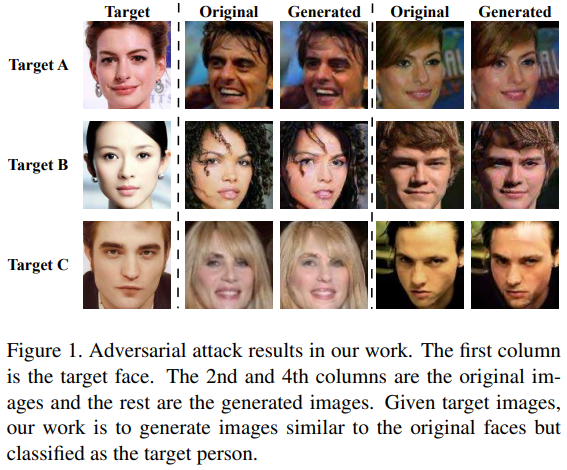
\includegraphics[width=0.90\textwidth]{img/p5m1.png} 
\caption{研究结果}
\label{Test}
\end{figure}

Szegedy et al 等人发现,目前对抗性攻击可以通过应用难以察觉的扰动来实现,这是人眼第一次难以观察到的扰动,而在 Szegedy 的工作之后,许多工作都集中在如何制作对抗性示例来攻击神经网络,使神经网络逐渐受到质疑。对抗性攻击的工作可以促进神经网络的发展,Akhtar 等人则回顾这些作品在现实世界场景中的贡献。在前人作品的启发下,该研究还对对抗性攻击进行了一些研究。大多数对抗性攻击旨在将分类器误导为错误标签,而不是确定的特定标签。

此外对图像分类器的攻击不能针对人脸识别网络,现有作品会对图像产生扰动,对面部进行一些化妆,并在面部添加眼镜、帽子或遮挡物。其对抗性例子是由不灵活的攻击算法固定的,而这些算法不能接受任何图像作为输入。该研究者的目标是生成与原始图像相似但可以分类为目标人的人脸图像,如图中所示,而直接操纵输入图像强度的方法是基于强度的。另外研究者的工作使用基于几何的方法来生成对抗样本。在该研究的工作中,研究者们使用生成对抗网络 (GAN) 来生成不受数据、算法或目标网络限制的对抗样本。

它可以接受任何人脸作为输入,并将其转换为对抗样本以进行攻击。为了生成对抗样本,该工作提出了 $A_{3}GN$ 来生成外观与原点相似但能够被归类为目标人的假图像。在人脸验证领域,两张人脸是否属于一个人是基于最后一层特征图之间的余弦距离,而不是基于每个类别的概率。所以 $A_{3}GN$ 更加关注人脸特征分布的探索。为了获取实例信息,该研究引入了条件变分自动编码器来从目标人脸中获取潜在代码,同时提供了注意力模块来捕获目标人脸的更多特征表示和脸部依赖关系。对于对抗样本,$A_{3}GN$ 采用了两种判别器——一个用于估计生成的人脸是否真实,称为正常判别器,另一个用于估计生成的人脸是否可以分类为目标人,称为实例判别器。

同时,引入余弦损失以保证假图像可以被目标模型分类为目标人物。研究者的主要贡献可以概括为三方面:

\begin{itemize}
\item [-] 研究者专注于攻击最先进的人脸识别网络的新方法。他们会被误导,将某人识别为目标人,而不是根据特征图而不是概率在人脸验证中不明显地错误分类。
\item [-] 引入 GAN 以生成与传统基于强度的攻击不同的对抗性示例。同时,这项工作提出了一种名为 $A_{3}GN$ 的新 GAN,用于生成与原点相似但与目标人脸具有相同特征表示的对抗样本。
\item [-] $A_{3}GN$ 的良好表现可以通过一组评估标准在身体相似度、相似度得分和识别准确度方面表现出来。
\end{itemize}

\subsection{根据影片深度伪造检测}

Marra F 等人 \cite{marra2018detection} 在其 Detection of GAN-generated fake images over social networks 的工作中得出,社交网络上虚假图像和视频的传播是一个快速增长的问题,商业媒体编辑工具允许任何人删除、添加或克隆人和对象,以生成虚假图像。已经提出了许多技术来检测这种传统的伪造品,但新的攻击每天都在出现。基于生成对抗网络 (GAN) 的图像到图像转换似乎是最危险的方法之一,因为它允许人们以非常现实的方式修改图像的上下文和语义。在该研究中,研究者们研究了几种图像伪造检测器对图像到图像转换的性能,无论是在理想条件下,还是在存在压缩的情况下,通常在上传到社交网络时执行。该研究在 36302 张图像的数据集上进行,表明传统和深度学习检测器都可以实现高达 95\% 的检测精度,但只有后者在压缩数据上保持高达 89\% 的高精度。

\begin{figure}[htb]
\centering 
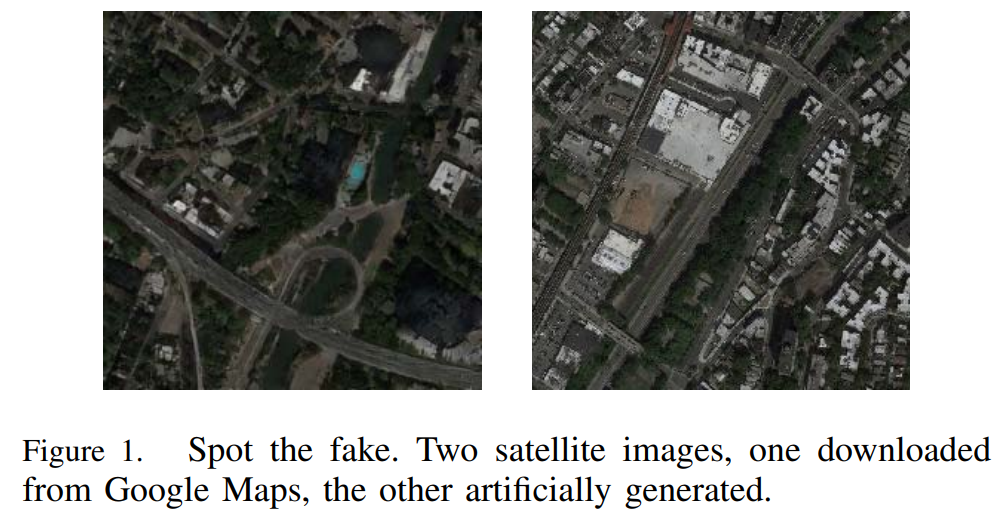
\includegraphics[width=0.90\textwidth]{img/p6m1.png} 
\caption{识别假货。两张卫星图像,一张是从谷歌地图下载的,另一张是人工生成的}
\label{Test}
\end{figure}

随着社交网络的扩散,传播信息和篡改的传播信息变得非常容易,其假新闻通常由多媒体内容支持,旨在提高其可信度。事实上,通过使用强大的图像编辑工具,例如 Photoshop 或 GIMP,即使是非专业用户也可以轻松地修改图像以获得逼真的结果,从而避开人类观察者的审查。最近发表在 Cognitive Research 上的一项研究试图通过视觉检查来衡量人们识别照片是否被篡改的能力。只有 62\%-66\% 的照片被正确分类,而且用户在定位操作方面表现得更差。在一项类似的研究中,只有 58\% 的图像被正确分类,并且只有 46\% 的经过处理的图像被正确分类,而广泛的图像伪造所代表的威胁刺激了多媒体取证的深入研究。结果,在适当的假设下,自动算法可以实现比人类更好的检测性能,例如在第一届 IEEE 图像取证挑战赛中,通过机器学习方法和经过适当训练的分类器获得了超过 90\% 的检测精度。

同时对于计算机生成的虚假图像,情况几乎相反,最近的一项研究证明,对于此类图像,人类的判断明显优于机器学习,这可能归因于当前的计算机图形工具无法提供良好的照片级真实感。因此该领域的研究活动较少,一些论文提出基于从小波分解或残差图像中提取的统计数据来检测计算机图形图像,而其他论文依赖于记录设备引入的不同噪声、色差痕迹或去马赛克滤波器的痕迹。探讨了颜色分布的差异,而在局部边缘块的统计特性中则用于区分,人脸不对称被提出作为区分计算机从自然人脸生成的判别特征。直到最近深度学习才被用于这项任务,并被发现优于以前的方法。因此,当虚假图像很容易被人类检测到时,对复杂检测器的需求就不那么迫切了。然而,计算机图形技术发展迅速,观察者发现越来越难以区分计算机生成的图像和摄影图像。事实上,最近已经设计出基于计算机图形的新形式的图像处理,其特点是更高水平的照片写实。

\begin{figure}[htb]
\centering 
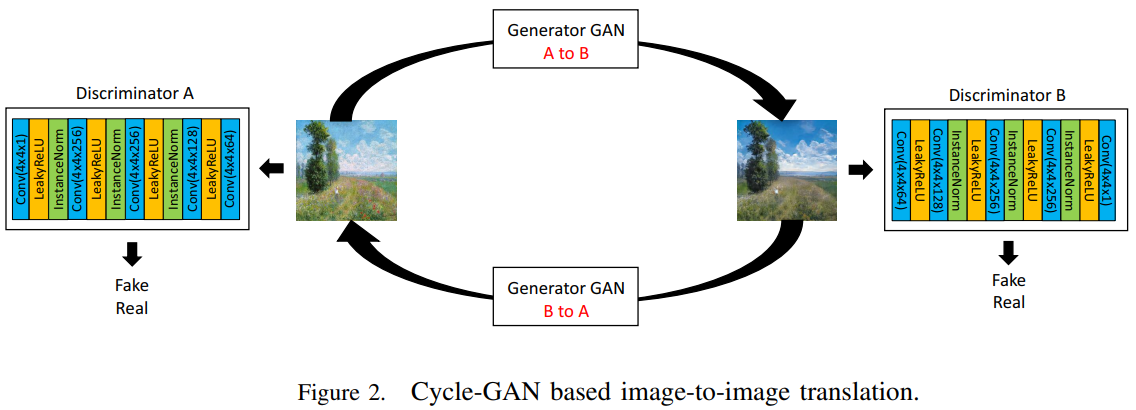
\includegraphics[width=0.90\textwidth]{img/p6m2.png} 
\caption{基于 Cycle-GAN 的图像到图像转换}
\label{Test}
\end{figure}

特别是,研究者在这里关注图像到图像的转换,这是一个通过将场景的一种可能表示转换为另一种表示来修改目标图像属性的过程,随着生成对抗网络 (GAN) 的出现,这种攻击变得相对容易且非常流行。其目的是生成与从给定来源绘制的真实图像无法区分的图像,研究者图中提供了图像到图像转换的示例。在这项工作中,研究者分析了许多基于学习的方法在检测图像到图像转换中的性能,其目标是了解这些攻击是否、在何种程度上以及在何种条件下可以被揭露。

为此研究者将考虑几种解决方案,这些解决方案既基于从图像取证文献中获取的最先进的方法,也基于针对该任务进行适当训练的通用非常深的卷积神经网络 (CNN)。同时研究者还将研究通过社交网络(如 Twitter)发布图像的情况。事实上,这既是最常见也是最具挑战性的情况,因为在图像上传时常规执行的压缩往往会削弱伪造检测器的性能。最后研究者将参考 J. Y. Zhu 等人提出的方法,描述本文分析的图像的生成过程,介绍用于检测的方法,最后讨论实验结果。

最后该研究提出了一项关于检测由基于 GAN 的图像到图像转换操作的图像的研究,比如一些检测器在原始图像上的表现非常好,但其中一些在类似 Twitter 的压缩图像上表现出明显的缺陷。深度网络可以更好地保持鲁棒性,尤其是 XceptionNet,即使在训练-测试不匹配的情况下,它也能保持相当好的工作。

\section{区块链进行视频追踪}

Hasan HR 等人 \cite{hasan2019combating} 在面对深度伪造的挑站下,在其 Combating deepfake videos using blockchain and smart contracts 认为,随着人工智能 (AI) 和深度学习技术的兴起,近年来虚假数字内容激增。假镜头、图像、音频和视频(称为 deepfakes)可能是一种可怕且危险的现象,并且有可能通过提供虚假现实来改变真相并削弱信任,数位媒体的真实性证明 (PoA) 对于帮助消除伪造内容的流行至关重要,而当前的解决方案缺乏提供数字媒体的历史跟踪和出处的能力。

\begin{figure}[htb]
\centering 
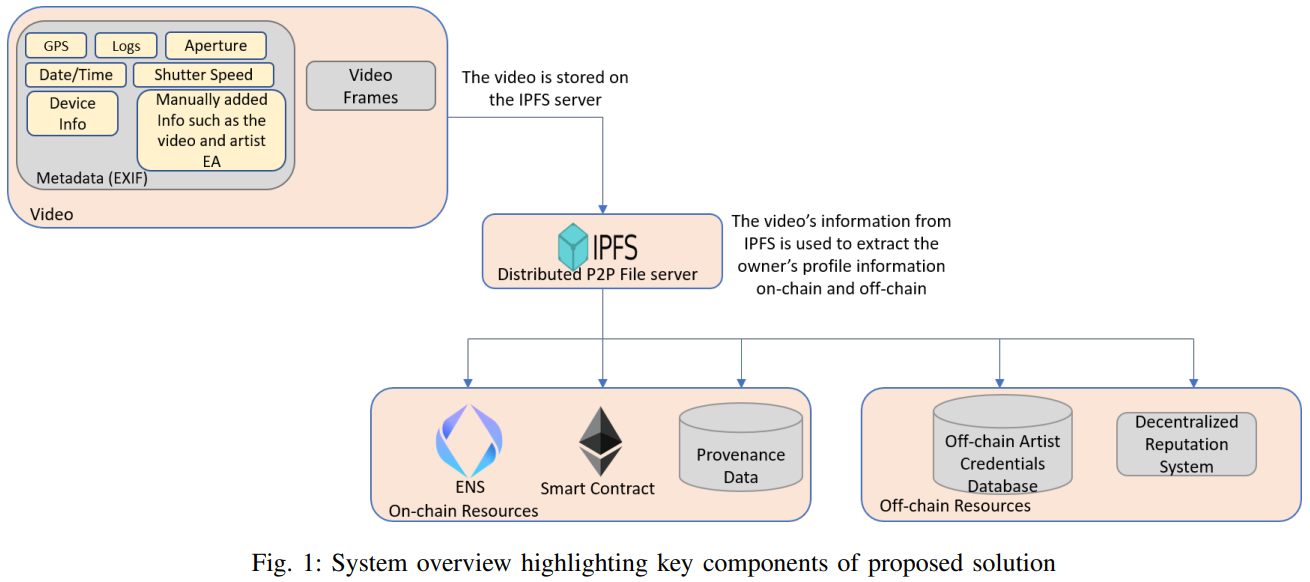
\includegraphics[width=0.90\textwidth]{img/p7m1.png} 
\caption{系统概述}
\label{Test}
\end{figure}

在该研究中,研究者们提供了一个解决方案和一个通用框架,使用以太坊智能合约来追踪和跟踪数字内容的出处和历史到其原始来源,即使数字内容被复制多次,其智能合约利用用于存储数字内容及其元数据的行星际文件系统 (IPFS) 的哈希值。解决方案专注于视频内容,且此研究提供的解决方案框架足够通用,可以应用于任何其他形式的数位内容。其解决方案依赖于这样一个原则,即如果内容可以可靠地追溯到可信或有信誉的来源,那么内容就可以是真实的和真实的。

拥有检测、打击和打击可能包括假视频、图像、绘画、音频等的 deepfake 数字内容的技术至关重要。如果有一种可靠、安全和值得信赖的方式来追溯数字内容的历史,那么实现这一目标并不难,其用户应有权访问数字内容的可信数据来源,并能够追溯历史项目以证明其原创性和真实性,而这种机制可以帮助用户避免被欺骗或诱骗相信虚假的数字内容。当前的解决方案可用于证明物理(而非数字)艺术品的真实性。以购买艺术品时会获得一份真品证书 (COA) 来说,有可能伪造此证书或发现它未从已知且受信任的机构签名的可能,同时从二级市场购买的艺术品更难证明其来源。

目前寻求的唯一方法是手动向画廊或产品来源询问他们从以前的所有者那里获得的 COA 以及他们的收据。在某种程度上,买家需要做大量的手工工作和检查才能获得准确的艺术品出处。到目前为止,还没有确定的方法来检查在线发布或发布的数字视频、音频或图像的原创性。将此类数字内容纳入 COA 的想法是不可行的。以可信和可信的方式确定发布的数字项目的真实来源是极其困难的,而一个典型的用户通常使用在线搜索引擎试图在数字媒体上找到相关的帖子、博客或评论,以判断其真实性,也因此非常需要用于在线数字内容的真实性证明 (PoA) 系统,以识别可信的发布来源,从而能够打击深度伪造的视频、音频和图像。

该研究提出了一个使用颠覆性技术区块链的去中心化真实性证明 (PoA) 系统,其区块链有能力在去中心化的分布式账本中提供不可变和防篡改的数据和交易。 ,同时区块链的适用性是巨大的,该技术有望在金融、食品行业、供应链管理、健康管理、物联网等许多企业、行业和领域发生变革和影响。而且区块链具有提供关键功能的能力,可用于以分散、高度可信和安全的方式证明数字资产的真实性和原创性。

\begin{figure}[htb]
\centering 
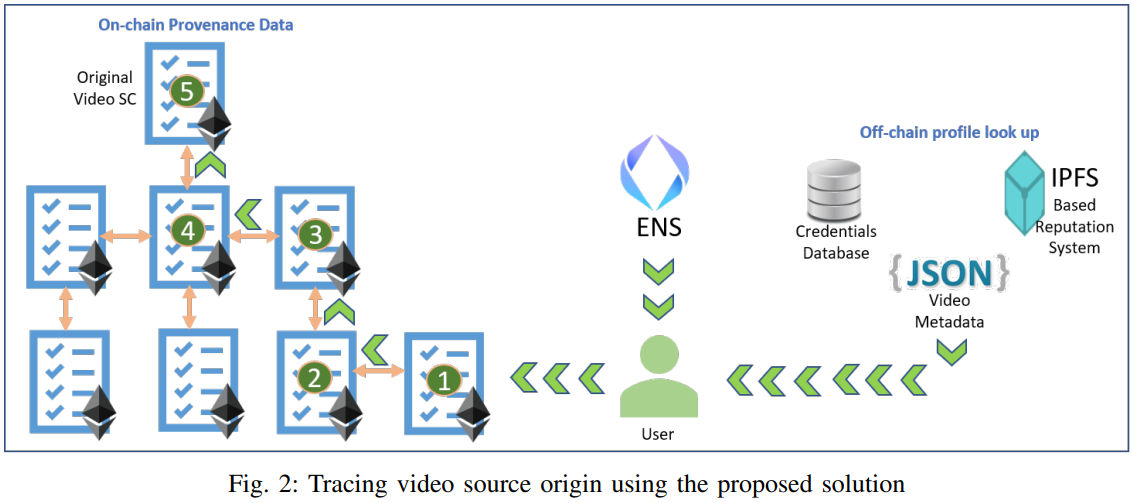
\includegraphics[width=0.90\textwidth]{img/p7m2.png} 
\caption{跟踪视频源来源}
\label{Test}
\end{figure}

S. Singh 等人,K. Biswas 等人,具有防篡改记录、日志和交易,在无许可区块链的情况下对所有人公开访问,或者在许可区块链的情况下仅限于某些参与者。对于 Deepfakes,无许可或公共区块链是最合适的。研究者在该研究中的解决方案基于带有智能合约的公共以太坊区块链,以管理和捕获对数字内容进行的交易历史,同时研究者提出了一种基于区块链的解决方案和一个通用框架,用于证明可能包括视频、音频、图像等的数字资产的真实性,其解决方案允许公开访问、可信和可信的数据来源,并跟踪和追溯已发布的在线视频的历史记录。而且此解决方案专注于视频内容,但本文提供的解决方案框架足够通用,可以应用于任何其他形式的数字内容,如音频和图像。

最后该研究提出了一种基于区块链的解决方案,用于证明数字视频的真实性,其中可以以分散的方式建立对原始视频创建者或来源的安全和可信的可追溯性。同时解决方案利用了去中心化存储系统 IPFS、以太坊名称服务和去中心化信誉系统,并提出的解决方案框架、系统设计、算法、序列图以及实现和测试细节足够通用,可以应用于其他类型的数字内容,例如音频、照片、图像和手稿,另外解决方案可以帮助用户确定视频或数字内容是否可追溯到可信且有信誉的来源,从而帮助打击 deepfake 视频和音频。

如果视频或数字内容不可追踪,则数字内容不可信任,其基于智能合约的解决方案为二级艺术家请求原始艺术家复制和编辑视频的许可提供了一种值得信赖的方式,而且智能合约的完整代码已在 Github 上提供,同时智能合约的关键特性和功能已经过适当的测试。研究者讨论了该研究的解决方案如何满足安全要求,以及如何抵御常见的安全攻击。在真实的以太坊网络上部署智能合约时,研究者估计了以太坊和天然气的运营成本,其成本估算是最低的,每笔交易始终低于 0.095 美元。作为未来的工作,研究者正在为用户开发前端 DApp,以自动建立已发布视频的真实性证明。同时还计划开发一个可插拔的 DApp 组件,以便在 Web 浏览器中播放或显示视频时提供可追溯性并建立真实性,其设计和实施功能齐全且可操作的分散信誉系统的工作也在进行中。



%\section{系统分析}
%\section{系统概念}
%\subsubsection{SSS1}

%\begin{itemize}
%\item [-][7,7] 空间卷积到 1*1*2048 然后一维卷积到 1*1*128
%\item [-]池化层到 1*1*2048 然后一维卷积到 1*1*128
%\end{itemize}


%\begin{itemize}
%\item Calculus
%\item Linear Algebra
%\item Basic Computer Concepts
%\end{itemize}

%\begin{description}
% \item[First] \hfill \\
% The first item
% \item[Second] \hfill \\
% The second item
% \item[Third] \hfill \\
% The third etc \ldots
%\end{description}

	\chapter{工作总结}
\label{chap:2}

本作业针对近年个人信息隐私保护等重要性日渐提升等原因,同时在面对近年来深度伪造等技术的发展带来对假讯息流通的挑战,对此针对该领域,在其检测与对抗性等工作进行梳理,同时在此说明近期的研究成果,其包含了多模态多尺度(Multi-modal Multi-scale) 和增量学习 (Incremental Learning) 所导入于检测领域的应用,另外也针对为了保护个人隐私所针对的语音检测对抗性跟应对语音攻击的深度伪造在语音检测与对抗性部分的研究进行整理,此外则是针对深度伪造在生成与检测的对抗性的部分针对两个不同的型态进行说明,最后则是因近年来深度伪造的成长,而讨论运用区块链对其视频进行追踪的手段的工作,将其作为在深度伪造与检测跟对抗性领域的安全措施进行说明。


%\begin{figure}[htb]
%\centering 
%\includegraphics[width=0.80\textwidth]{img/XXXXX.png} 
%\caption{XXXX}
%\label{Test}
%\end{figure}


%\begin{itemize}
%\item [-] L1
%\end{itemize}

%\begin{Verbatim}
%CODE
%\end{Verbatim}



%\begin{figure}[htb]
%\centering 
%\includegraphics[width=0.60\textwidth]{img/picname.png} 
%\caption{XXXX}
%\label{Test}
%\end{figure}


    \appendix
    \printbibliography[heading = bibintoc]
    
    % 如有需要使用研究生成果页
    \def\cpublication{攻读硕士期间发表的论文及其他成果}

%\renewcommand{\bibname}{\cpublication}
%\begin{thebibliography}{9}{
%\zihao{5}
%\bibitem{publish} 
%\textbf{扎克·施耐德}, XXX XXX, et al. XXXX Title[C/OL]//III H D, SINGH A. Proceedings of Machine Learning Research: Proceedings of the 37th International Conference on Machine Learning: vol. 119. [S.l.]: PMLR, 2020: XXXX-XXXX. http://proceedings.ml r.press/XXXX.html.(一作,CCF-A)
%}\end{thebibliography}
%\addcontentsline{toc}{chapter}{\cpublication}


	\backmatter
	\chapter{致谢}

非常感谢 刘宏 教授,在  课让XXXXXX,该工作也帮助到学生目前的开发与研究工作进度,同时也对目前深度伪造的进展有所调研,同时也将此流程在其他课程的作业上进行测试获得良好的回馈。最后感谢在这一年来一起寒窗苦读得同学与所有老师,还有默默在开源社群与前沿研究奉献的技术人员跟研究者们。
	% 需替换门户原创页pdf/扫描pdf
	%% Copyright (c) 2008-2009 solvethis
% Copyright (c) 2010-2017,2021 Casper Ti. Vector
% Copyright (c) 2021 Kurapica
% Copyright (c) 2021 iofu728
% All rights reserved.
%
% Redistribution and use in source and binary forms, with or without
% modification, are permitted provided that the following conditions are
% met:
%
% * Redistributions of source code must retain the above copyright notice,
%   this list of conditions and the following disclaimer.
% * Redistributions in binary form must reproduce the above copyright
%   notice, this list of conditions and the following disclaimer in the
%   documentation and/or other materials provided with the distribution.
% * Neither the name of Peking University nor the names of its contributors
%   may be used to endorse or promote products derived from this software
%   without specific prior written permission.
%
% THIS SOFTWARE IS PROVIDED BY THE COPYRIGHT HOLDERS AND CONTRIBUTORS "AS
% IS" AND ANY EXPRESS OR IMPLIED WARRANTIES, INCLUDING, BUT NOT LIMITED TO,
% THE IMPLIED WARRANTIES OF MERCHANTABILITY AND FITNESS FOR A PARTICULAR
% PURPOSE ARE DISCLAIMED. IN NO EVENT SHALL THE COPYRIGHT HOLDER OR
% CONTRIBUTORS BE LIABLE FOR ANY DIRECT, INDIRECT, INCIDENTAL, SPECIAL,
% EXEMPLARY, OR CONSEQUENTIAL DAMAGES (INCLUDING, BUT NOT LIMITED TO,
% PROCUREMENT OF SUBSTITUTE GOODS OR SERVICES; LOSS OF USE, DATA, OR
% PROFITS; OR BUSINESS INTERRUPTION) HOWEVER CAUSED AND ON ANY THEORY OF
% LIABILITY, WHETHER IN CONTRACT, STRICT LIABILITY, OR TORT (INCLUDING
% NEGLIGENCE OR OTHERWISE) ARISING IN ANY WAY OUT OF THE USE OF THIS
% SOFTWARE, EVEN IF ADVISED OF THE POSSIBILITY OF SUCH DAMAGE.

{
	\ctexset{section = {
		format+ = {\centering}, beforeskip = {40bp}, afterskip = {15bp}
	}}
	\specialchap{北京大学学位论文原创性声明和使用授权说明}

	% 学校书面要求本页面不要页码,但在给出的 Word 模版中又有页码。
	% 此处以学校书面要求为准。
	\thispagestyle{empty}
	
	% 替换扫描pdf,去除includegraphics前注释
	\begin{textblock}{1}(-0.8,-0.08)
		\colorbox{white}{
			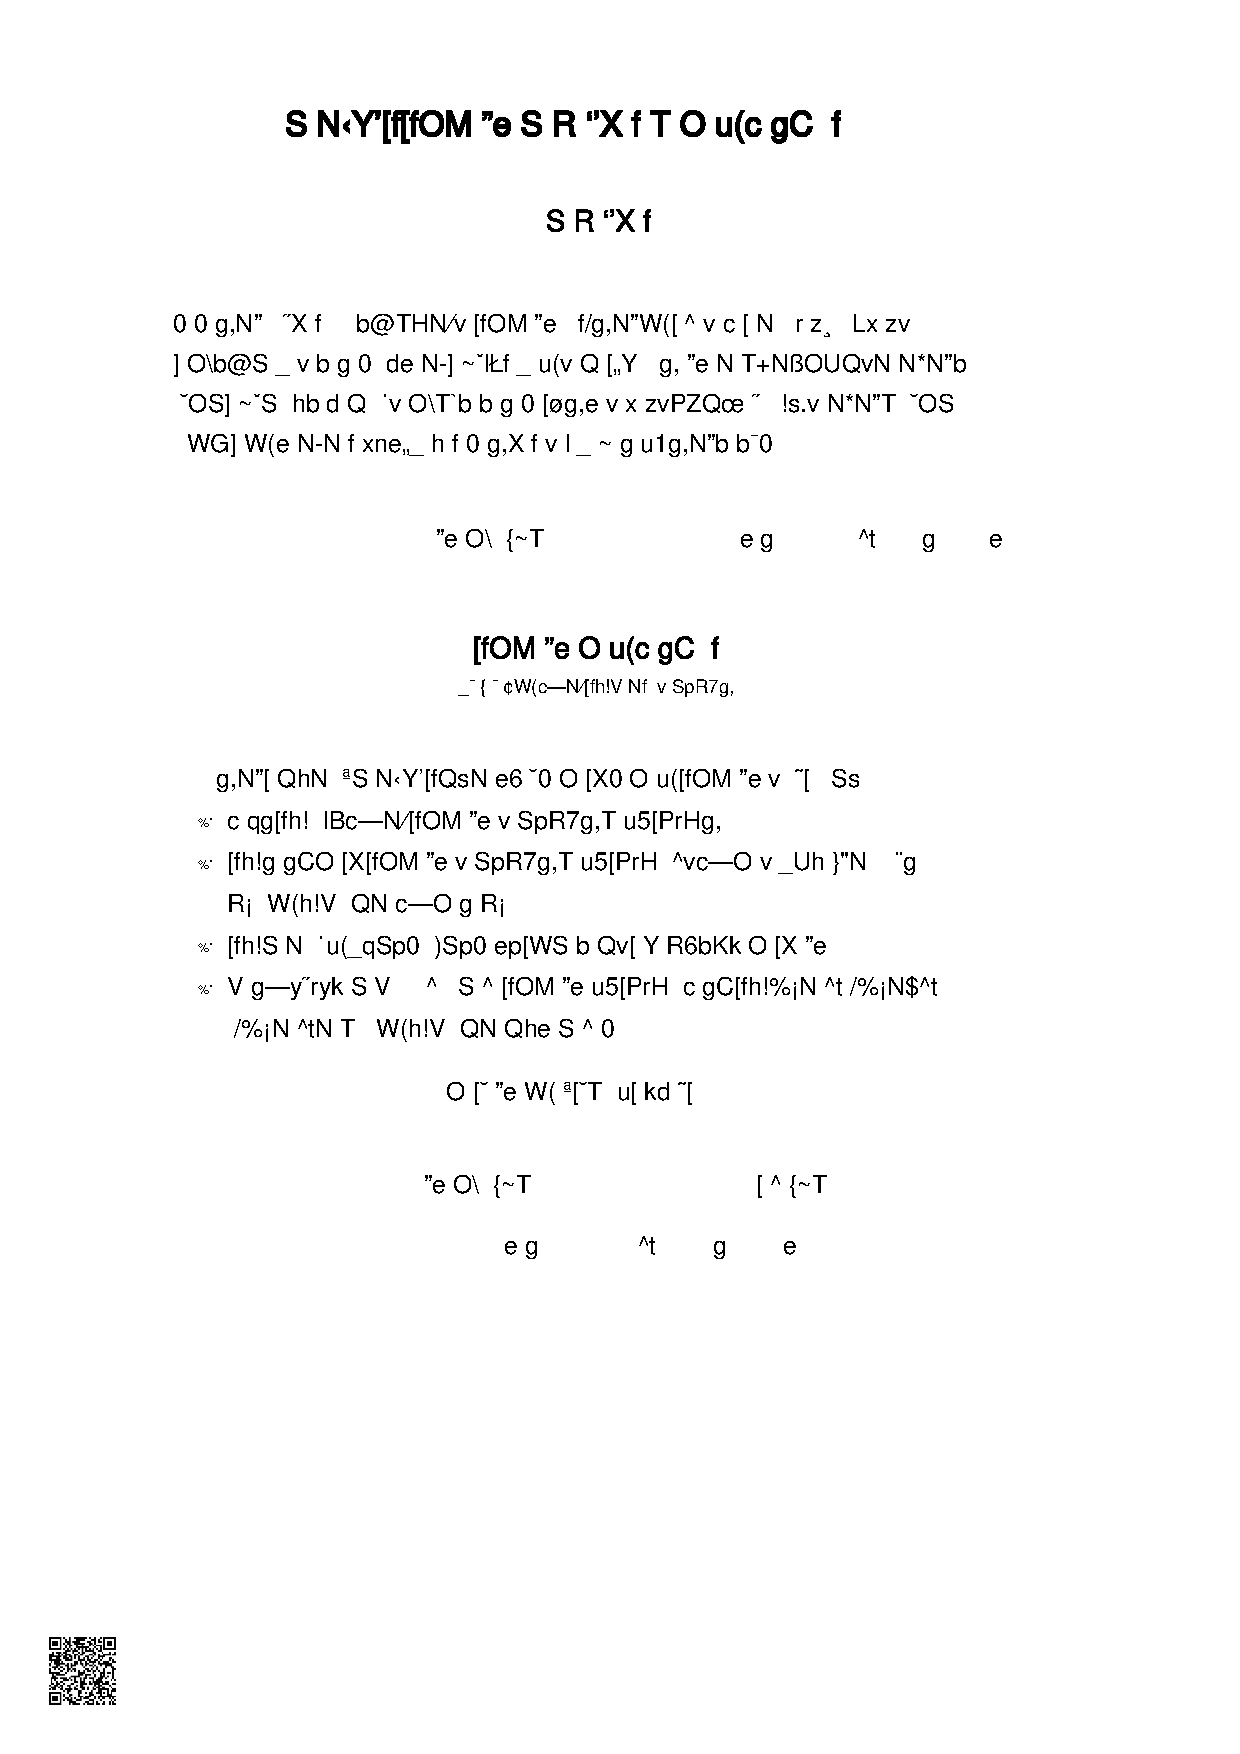
\includegraphics[height = 1.2448\textheight]{img/lwsm_180xxxxxxx.pdf}
		}
	\end{textblock}
}

% vim:ts=4:sw=4

\end{document}

% vim:ts=4:sw=4